\chapter{Preliminaries}
\label{chap:preliminaries}

% https://math.stackexchange.com/questions/566565/are-if-and-iff-interchangeable-in-definitions

%\paragraph{Notation}

When dealing with sets, we use the operator $+$ in place of $\cup$ if we want to emphasize that the operands are disjoint.
Similarly, we use the operator $-$ in place of $\setminus$ to stress that the right operand is a subset of the left operand.
We sometimes use set elements where sets would be mathematically correct, \eg{} $\{1,2\} + 3 = \{1,2,3\}$.
This is to be interpreted as the element being wrapped in a set implicitly.


\paragraph{Graphs}

A \emph{(simple, undirected) graph} $G$ is a tuple $G = (V, E)$ of \emph{vertices} $V$ and \emph{edges} $E \subseteq \left\{\{u,v\} \vert (u,v) \in V^2 \right\}$.
For an arbitrary graph $H$ we sometimes denote its vertices by $V(H)$ and its edges by $E(H)$.
Graphs can be weighted, assigning real-values weights to its vertices and/or edges.
We differentiate between vertex-weighted graphs that provide a weight function $w_v \colon V \to \mathbb{R}$ and edge-weighted graphs that provide a weight function $w_e \colon E \to \mathbb{R}$.
When graphs are weighted, we typically include the weight functions in the graph tuple, \eg{} $G_w = (V,E,w_v)$.
Of course, graphs can be both vertex- and edge-weighted.

Given a graph $G = (V, E)$, two vertices $u, v \in V$ are said to be \emph{adjacent} if there's an edge connecting $u$ to $v$, \ie{} $\{u, v\} \in E$.
Adjacent vertices are also called \emph{neighbors}.
A vertex $v$'s \emph{degree} $\deg(v)$ is the number of vertices that are adjacent to it, \ie{} $\deg(v) \coloneqq \abs{\{u \vert \{u,v\} \in E\}}$.
An edge $\{u, v\} \in E$ is said to be \emph{incident} to its \emph{endpoints} $u$ and $v$.

A \emph{path} $p$ is a (nonempty) sequence of edges that connects a sequence of distinct vertices $(v_1, \dots, v_n)$, \ie{} $p = (\{v_1, v_2\}, \dots, \{v_{n-1},v_n\}) \land \forall i \neq j \colon v_i \neq v_j$.
The first and last vertices $v_1, v_n$ of a path are called its \emph{endpoints}.
A path $p$'s \emph{length} is the number of edges in the path.

A graph $G = (V, E)$ is \emph{connected} if there exists a path between any pair of vertices in the graph.
$G$ is said to be \emph{$k$-(vertex)-connected} if one needs to remove $k$ or more vertices and their incident edges to disconnect $G$.
Graphs that are 2-vertex-connected are also called \emph{biconnected}.

A \emph{subgraph} $H$ of a graph $G$, denoted $H \subseteq G$ is a graph with a subset of vertices and edges from $G$, \ie{} $V(H) \subseteq V(G)$ and $E(H) \subseteq E(G)$.
A subgraph is said to be \emph{spanning} if it includes all vertices of the original graph, \ie{} $V(H) = V(G)$.


\paragraph{Graph Clustering}

Given a graph $G = (V, E)$, a \emph{clustering} $\mathcal{C}$ of $G$ is a partition $\mathcal{C} = \{C_1, \dots, C_k\}$ of its vertices $V$ into non-empty, pairwise disjoint \emph{clusters} of vertices, \ie{} $\bigcup_{i=1}^k C_i = V$, $\forall i \colon C_i \neq \varnothing$, and $\forall i \neq j \colon C_i \cap C_j = \varnothing$.

A clustering $\mathcal{C} = \{ C_1, \dots, C_k \}$ of a graph $G$ induces a so-called \emph{cluster graph} of $G$, a vertex- and edge-weighted graph $G_\mathcal{C} = (V_\mathcal{C}, E_\mathcal{C}, w_v, w_e)$ whose vertices are the clusters $C_i$:
%
\begin{align*}
V_\mathcal{C} &\coloneqq \{ C_1, \dots, C_k \} \\
E_\mathcal{C} &\coloneqq \{ \{C_i, C_j\} \vert (C_i, C_j) \in \mathcal{C}^2, C_i \neq C_j \} \\
w_v(C_i) &\mapsto \abs{C_i} \\
w_e(\{C_i, C_j\}) &\mapsto \abs{\{ (u,v) \in E \vert u \in C_i \land v \in C_j \}}
\end{align*}



\paragraph{Graph Operations}

% https://en.wikipedia.org/wiki/Homeomorphism_(graph_theory)#Subdivision_and_smoothing

Given a graph $G = (V, E)$, one can \emph{subdivide} an edge $e \coloneqq \{u,v\} \in E$ by removing the edge $e$ and inserting a new vertex $w$ with edges to both $u$ and $v$.
This produces a graph $G^\prime = (V^\prime, E^\prime)$ with $V^\prime = V + w$ and $E^\prime = E - \{u,v\} + \{u,w\} + \{w,v\}$.
A graph $H$ is said to be a \emph{subdivision} of $G$ if $H$ can be obtained from $G$ by repeatedly subdividing edges.
$H$ is a \emph{1-subdivision} of $G$ if it can be obtained from $G$ by subdividing every edge exactly once.

One can also \emph{contract} an edge $\{u,v\}$ of a graph $G = (V, E)$ if its endpoints $u$ and $v$ don't have any neighbors in common, deleting the edge and \quoted{merging} its endpoints into a new vertex $w$.
This removes the edges $E_- \coloneqq \{ \{x,y\} \in E \vert u \in \{x,y\} \lor v \in \{x,y\} \}$ and creates new edges $E_+ \coloneqq \{ \{w,x\} \vert \{u,x\} \in E \lor \{v,x\} \in E \}$, producing a new graph $G^\prime = (V^\prime, E^\prime)$ with $V^\prime = V - u - v + w$ and $E^\prime = E - E_- + E_+$.
Similarly, a vertex $v$ of degree 2 can be \emph{smoothed}, replacing it and its incident edges with a new edge $\{u,w\}$ between its original neighbors $u$ and $v$, \ie{} $G^\prime = (G^\prime, E^\prime)$ with $V^\prime = V - v$ and $E^\prime = E - \{u,v\} - \{v,w\} + \{u,w\}$.



\paragraph{Graph Drawings}

% Drawing
% https://proofwiki.org/wiki/Definition:Adjacent_(Graph_Theory)/Faces

A \emph{drawing} $\Gamma$ of a graph $G = (V, E)$ maps its vertices to distinct points in the plane and its edges to continuous curves between its endpoints in the plane.
The graph $G$ is called \emph{planar} if it permits a drawing in which its edges don't self-intersect and don't cross other edges, \ie{} the graph's edges only intersect in shared endpoints.
Such a drawing is called a \emph{planar drawing} of $G$.
If all edges of $G$ are line segments, we also call it a \emph{planar straight-line drawing}.

A planar drawing $\Gamma$ of a graph $G$ partitions the plane into mutually disjoint regions called \emph{faces}.
All faces but one, the \emph{internal faces}, are bounded; the unbounded face is called the \emph{outer face}.
Faces are identified by the cyclic order of vertices that are encountered when walking on its boundary \cite{angelini2015monotone} in such a way that the bounded area lies on the left side of the boundary.
Vertices and edges are said to be \emph{incident} to a face if they lie on the face's boundary.
Similarly, two faces are said to be \emph{adjacent} if there exists an edge they are both incident to.
If vertices or edges lie on the boundary of outer face, they are said to be \emph{external}, otherwise they are \emph{internal}.

% Planar Embedding

A \emph{planar embedding} $\phi$ of $G$ is an equivalence class of planar drawings that define the same set of faces for $G$.
A planar embedding $\phi$ therefore uniquely determines the internal faces and the outer face, or, equivalently, the cyclic order of the edges incident to each vertex in addition to the choice of the outer face \cite{angelini2015monotone}.

We also use the term \emph{plane graph} to refer to planar graph $G$ in combination with a planar embedding $\phi$ and denote it as $G_\phi$. A plane graph $G$ can be \emph{face-weighted} if there's a weight function $w_f \colon F_\text{int}(G) \to \mathbb{R}$ assigning real numbers to its internal faces $F_\text{int}(G)$.

% Triangulatedness

A planar graph $G$ is said to be \emph{maximal} or \emph{triangulated} if adding any edge to $G$ would result in a nonplanar graph.
Thus, in a maximal plane graph, all faces, including the outer face, are triangles.
Similarly, a plane graph $G_\phi$ is said to be \emph{internally triangulated} if all internal faces are triangles.

A \emph{multigraph} is a graph that, as opposed to a simple graph, can have multiple edges between a pair of vertices as well as so-called loops, \ie{} edges connecting a vertex to itself.
The \emph{dual (graph)} $G_\phi^*$ of a plane graph $G_\phi$ is a plane multigraph that has a vertex $v_f$ for every face $f$ of $G_\phi$ and edges connecting the vertices corresponding to the incident faces of each edge in the graph $G_\phi$.
The dual is embedded in such a way that the cyclic order of the edges incident to each vertex is equivalent to the cyclic order of the edges bounding the respective faces in the original graph.
In relation to the dual $G_\phi^*$, the original graph $G_\phi$ is also called the \emph{primal (graph)}.
The \emph{weak dual} $G_\phi^-$ of a plane graph $G_\phi$ is its dual without the vertex corresponding to the $G_\phi$'s outer face \cite{fleischner1974}.

\begin{figure}[H]
	\centering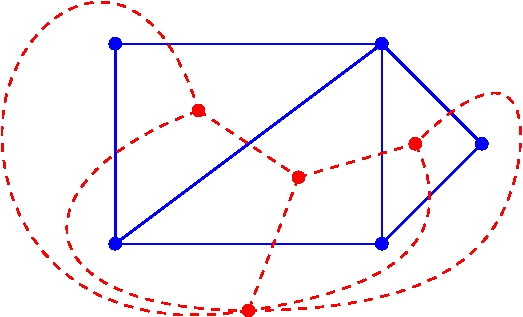
\includegraphics[height=130px]{Resources/Preliminaries-Dual.pdf}
	\caption{A plane graph $G$ (in blue) and its dual $G^*$ (in red).}
	\label{fig:preliminaries-dual}
\end{figure}

An example for a plane graph and its dual is illustrated in \cref{fig:preliminaries-dual}.
Forming the dual of a plane graph essentially turns vertices into faces and vice versa and \quoted{rotates} the edges of the plane graph as illustrated in \cref{fig:preliminaries-dual}.
Note that the planar embedding of the dual graph is uniquely determined by the planar embedding of its primal.
When forming the dual of the dual of a plane graph, we get back the original plane graph, \ie{} $(G^*)^* = G$.



\paragraph{Contact Representations}

In a \emph{(simple) contact representation} of a plane graph $G_\phi$, the vertices are represented by pairwise internally disjoint regions in the plane and edges are implicitly defined by the non-trivial contacts between the corresponding regions \cite{alam2013linear}.
Because $G_\phi$ is simple, the regions corresponding to adjacent vertices in $G_\phi$ must therefore only share a single continuous boundary in the contact representation.
A contact representation is said to be \emph{hole-free} if all regions other than the unbounded outer region have a corresponding vertex in $G_\phi$.

Unless otherwise noted, we assume that contact representations are hole-free and that they respect the original graph $G_\phi$'s embedding, \ie{} for all regions, the cyclic order of the boundaries with adjacent regions is equivalent to the cyclic order of the incident edges of the corresponding vertex in $G_\phi$ and its neighbors.

Given a plane graph $G_\phi$, a contact representation of $G_\phi$ with axis-aligned rectilinear polygons is called a \emph{rectilinear dual} of $G_\phi$ \cite{alam2013computing}.
The name \quoted{dual} is fitting here because vertices of the original graph turn into faces, or regions, of the rectilinear dual.
In fact, we can regard the rectilinear dual as a plane graph itself: the polygons' corners are vertices, connected by edges as determined by the polygons' sides, as illustrated in \cref{fig:preliminaries-rectilinear-dual}.
We use the term rectilinear dual to refer to the the actual arrangement of rectilinear polygons and the induced plane graph interchangeably.

\begin{figure}[H]
	\centering
	\subfigure[]{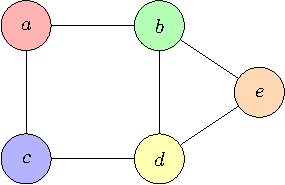
\includegraphics[height=90px]{Resources/Preliminaries-RectilinearDual-Primal.pdf}}
	\quad
	\subfigure[]{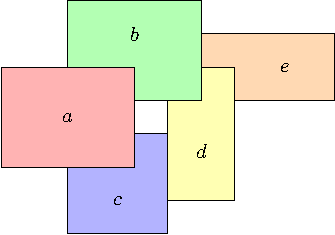
\includegraphics[height=90px]{Resources/Preliminaries-RectilinearDual-Polygons.pdf}}
	\quad
	\subfigure[]{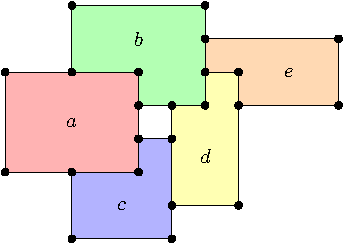
\includegraphics[height=90px]{Resources/Preliminaries-RectilinearDual-Dual.pdf}}
	\caption{A plane graph $G_\phi$ (a) and a possible rectilinear dual of $G_\phi$ with a hole, as a plain arrangement of polygons (b), and construed as yet another plane graph (c).}
	\label{fig:preliminaries-rectilinear-dual}
\end{figure}

A contact representation can be \emph{weighted}, assigning a real weight to all regions corresponding to vertices of its primal.
We define the \emph{normalized cartographic error} \cite{alam2015quantitative} of a weighted contact representation as
%
\begin{equation*}
    \max\limits_{v \in V(G)} \frac{\abs{A^\prime(v) - w(v)}}{\max\{A^\prime(v),w(v)\}},
\end{equation*}
%
where $w(v)$ is the prescribed area of the region corresponding to vertex $v$ and $A^\prime(v)$ is its actual area $A(v)$, normalized such that constant factors drop out, \ie{}
%
\begin{equation*}
	A^\prime(v) \coloneqq A(v) \cdot \frac{\sum\limits_{u \in V}{w(u)}}{\sum\limits_{u \in V}{A(u)}}.
\end{equation*}
%
We say that a weighted contact representation is \emph{$\varepsilon$-area-proportional} if its normalized cartographic error is less than or equal to $\varepsilon$.



\paragraph{Area Universality}

A plane graph $G$ with internal faces $F_\text{int}$ is \emph{area universal} if, for every area assignment of its internal faces $A \colon F_\text{int} \to \mathbb{R}_+$, there exists a planar straight-line drawing of $G$ with the same embedding such that all internal faces $f \in F_\text{int}$ have the area $A(f)$ prescribed by $A$.

Recall that Thomassen \cite{thomassen1992plane} showed that all (planar embeddings of) cubic graphs, \ie{} graphs in which all vertices have degree 3, are area-universal, and that Kleist \cite{kleist2019planar} showed that all plane 1-subdivisions of planar graphs are area-universal, too.
